\documentclass[aspectratio=169,xcolor=dvipsnames]{beamer}
\usetheme{SimplePlus}

% Links
\usepackage{hyperref}
\hypersetup{
    colorlinks=true,
    linkcolor=blue,
    filecolor=magenta,      
    urlcolor=brown,
    linkbordercolor=1 1 1,
    citebordercolor=1 1 1,
    linkbordercolor=1 1 1,
    menubordercolor=1 1 1,
    urlbordercolor=1 1 1,
}

% images
\usepackage{graphicx} 

%
\usepackage{booktabs} % Allows the use of \toprule, \midrule and \bottomrule in tables


\title[short title]{\textbf{Robot Mazes}} 
\subtitle{Project I Checkpoint - Artificial Inteligence}

\author[Marcelo  Francisco] {\textbf{Grupo 21} \\ \begin{tabular}{r l} 
	\email{up201906086@up.pt} & Marcelo Henriques Couto \\
	\email{up201907361@up.pt} & Francisco Pinto de Oliveira \\
\end{tabular}
}

\institute[FEUP] 
{
    Faculdade de Engenharia da Universidade do Porto
}
\date{\today} 



\begin{document}

\begin{frame}
    \titlepage
\end{frame}


\begin{frame}{Problem Description}
    Implement an Artificial Inteligence agent based on heuristic search methods to solve \href{https://erich-friedman.github.io/puzzle/robot/}{Robot Mazes} puzzle. 

    \vspace{0.5em}

    \begin{minipage}{0.62\textwidth}
        \begin{itemize}
            \item \textbf{Grid:} The puzzle is made up of a 5x5 grid, with a start and finish positions. Between each spot in the grid, there can be a wall.
            \item \textbf{Robot and Movement:} The robot is placed at the starting spot and can make a limited number of movements (Left, Right, Up or Down), depending on the puzzle. When there are no moves left, he will repeat the sequence chosen until he gets stuck or reaches the ending spot.
        \end{itemize}
    \end{minipage}%
    \begin{minipage}{0.38\textwidth}
        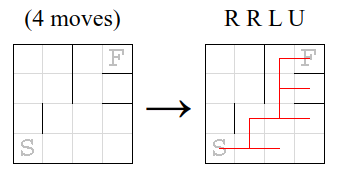
\includegraphics[width=50mm]{img/puzzle.png}
    \end{minipage}
    \begin{itemize}
            \item \textbf{Objective:} The objective is to, for a given puzzle, decide the correct sequence of movements for the robot to loop from start to finish.
    \end{itemize}
\end{frame}



\begin{frame}{Problem Formulation as a Search Problem}
    \textbf{State Representation:} With N being the number of moves allowed, state S is an array of size N of the movements chosen. \\
    \textbf{Initial State:} A random state. E.g. S = [Right,Up,Left,Down] \\
    \textbf{Objective Test:} The cycle of movements of the given state, repeated indefinitely, always changes position after an iteration and eventually reaches the goal spot. \\
    \textbf{Operators:}
    \begin{table}
        \begin{tabular}{l l l l}
            \toprule
            \textbf{Operator} & \textbf{Pre-Condition} & \textbf{Effect} & \textbf{Cost} \\
            \midrule
            ChangeMov(i,m)  & $ i >= 0 \land i < N \land S[i] \neq m $ & $S[i] = m $  & 1 \\
            \bottomrule
        \end{tabular}
        \caption{Operators}
    \end{table}
    
    With this approach, we consider every solution to be equally optimal, being the speed of the algorithm the desirable aspect to optimize.
\end{frame}




\begin{frame}{Implementation}
    \textbf{Language:} Python \\
    \textbf{Environment:} Anaconda \\
    \textbf{Dependencies:} pygame, pygame\_menu \\
    \textbf{Data Structures:} 
    \begin{enumerate}
        \item Map representing the positions of the walls in the maze - python \textit{dictionary}
        \item List representing the movements of the robot in sequence (state) - python \textit{list}
    \end{enumerate}\\
    \textbf{Algorithms:} Simulation of a given sequence of movements (state)\\
\end{frame}




\begin{frame}{Approach}
    \textbf{Heuristics}
    \begin{itemize}
        \item \textbf{Compare with shortest path}
        \begin{enumerate}
            \item Calculate shortest path from start to finish
            \item Simulate current solution 
            \item Compare the two paths. The closest to the shortest path the better the solution
            \item \textbf{Evaluation functions:} given $SP$ the shortest path from start to finish and $P$ the path made by the simulation:
            \begin{itemize}
                \item $length(SP) - length(SP.count(P))$, where $SP.count$ is the number of positions from $SP$ that are in $P$
            \end{itemize}
        \end{enumerate}
        \item \textbf{Manhattan Distance}
        \begin{enumerate}
            \item Simulate the current solution
            \item Calculate Manhattan Distance from where the robot got stuck to the goal
            \item \textbf{Evaluation functions:} given $f$ the function that gives the Manhattan Distance, $S$ the state and $SP$ the shortest path
            \begin{itemize}
                \item $f(S)$ - non admissible
                \item $f(S) / SP.size$ - admissible
            \end{itemize}
        \end{enumerate}
    \end{itemize}
    
\end{frame}


\begin{frame}{Approach}
    \textbf{Heuristics}
    \begin{itemize}
        \item \textbf{Max Distance}
        \begin{enumerate}
            \item Simulate the current solution
            \item Calculate Max Distance from where the robot got stuck to the goal ($max(distx_, dist_y)$)
            \item \textbf{Evaluation functions:} given $f$ the function that gives the Max Distance, $S$ the state and $M$ the maze
            \begin{itemize}
                \item $f(S)$ - non admissible
                \item $f(S) / M.size$ - admissible
            \end{itemize}
        \end{enumerate}
    \end{itemize}
    
    \textbf{Note:} The way we approached and interpreted the problem lead to a non-existance in comparison of solutions, as there is a fixed number of movements for each problem. For this matter, we chose to compare each solution simply through the speed of its attainance. Therefore, and because the closest solution to the root is not the only valid one, non admissible heuristics are acceptable. 
    
\end{frame}




\begin{frame}{Algorithms Implemented}
    \begin{itemize}
        \item \textbf{Breadth-First Search (BFS)} 
        \item \textbf{Depth-First Search (DFS)}
        \item \textbf{Iterative Deepening Search (IDS)}
        \item \textbf{Greedy Search}
        \item \textbf{A* algorithm}
    
    \end{itemize}
    
    As the cost of our operators is 1, \textbf{Uniform Cost Search} is equivalent to \textbf{Breadth-First Search}
    
    We did not give any limit in depth for either \textbf{Depth-First Search} or \textbf{Iterative Deepening Search}, as there is always a solution and we do not allow for repeated nodes/states.
    
\end{frame}
\begin{frame}{Results(Level 2)}
    \scalebox{0.8}{
        \begin{table}[]
            \centering
            \begin{tabular}{|l|l|l|l|}
            \hline
            \textbf{Algorithm} & \textbf{Execution Time} & \textbf{Iterations} & \textbf{Solution Depth} \\ \hline
            Breadth First Search & 28.76 & 143 & 4 \\ \hline
            Depth First Search & 19.64 & 92 & 92 \\ \hline
            Iterative Deepening DFS & 52.58 & 379 & 4 \\ \hline
            Greedy(Manhattan) & 11.25 & 8 & 5 \\ \hline
            A*(Manhattan) & 16.02 & 12 & 5 \\ \hline
            Greedy(Manhattan/Shortest Distance) & 9.04 & 8 & 5 \\ \hline
            A*(Manhattan/Shortest Distance) & 38.53 & 68 & 4 \\ \hline
            Greedy(Shortest Path) & 41.03 & 40 & 9 \\ \hline
            A*(Shortest Path) & 36.38 & 48 & 5 \\ \hline
            Greedy(Maximum Axis Distance) & 9.86 & 8 & 5 \\ \hline
            A*(Maximum Axis Distance) & 15.06 & 16 & 5 \\ \hline
            Greedy(Maximum Axis Distance/Maze Size) & 9.26 & 8 & 5 \\ \hline
            A*(Maximum Axis Distance/Maze Size) & 35.50 & 68 & 4 \\ \hline
            \end{tabular}
        \end{table}
    }
\end{frame}


\begin{frame}{Results(Level 8)}
    \scalebox{0.8}{
        \begin{table}[]
            \begin{tabular}{|l|l|l|l|}
            \hline
            \textbf{Algorithm} & \textbf{Execution Time} & \textbf{Iterations} & \textbf{Solution Depth} \\ \hline
            Breadth First Search & 972.04 & 3992 & 7 \\ \hline
            Depth First Search & 515.58 & 1868 & 1868 \\ \hline
            Iterative Deepening DFS & 10790.95 & 80064 & 9 \\ \hline
            Greedy(Manhattan) & 43.48 & 21 & 10 \\ \hline
            A*(Manhattan) & 75.63 & 44 & 8 \\ \hline
            Greedy(Manhattan/Shortest Distance) & 41.60 & 21 & 10 \\ \hline
            A*(Manhattan/Shortest Distance) & 1308.32 & 3368 & 7 \\ \hline
            Greedy(Shortest Path) & 38.89 & 17 & 8 \\ \hline
            A*(Shortest Path) & 234.00 & 144 & 9 \\ \hline
            Greedy(Maximum Axis Distance) & 75.57 & 39 & 12 \\ \hline
            A*(Maximum Axis Distance) & 423.44 & 602 & 8 \\ \hline
            Greedy(Maximum Axis Distance/Maze Size) & 76.28 & 39 & 12 \\ \hline
            A*(Maximum Axis Distance/Maze Size) & 1246.24 & 3368 & 7 \\ \hline
            \end{tabular}
        \end{table}
    }
    
\end{frame}

\begin{frame}{Conclusions}
    
    From the different approaches analyzed we were able to draw some conclusions:
    \begin{itemize}
        \item Despite our heuristic functions not being, at our eyes, closely related to the problem and meaningful, they proved to greatly improve our algorithms' performance.
        \item The results show that our admissible heuristics made the \textbf{A* algorithm} find the 'ideal solution', if that would be the solution closest to the root node. However, the non admissible heuristics improved its speed greatly.
        \item In our interpretation of the problem, any valid solution is acceptable and the best solution is the one simply achieved the fastest. In this case, the \textbf{Greedy algorithm} was the best, as it yielded a solution in the least time and iterations.
        \item \textbf{IDS} was a particularly bad approach, as the optimal was not necessary.
        \item \textbf{DFS} as shown the same number of iterations as depth, as, without any limits, because a solution can always be reached through a certain branch, it will not backtrack ever, being effectively a brute-force approach.
    \end{itemize}

\end{frame}

\begin{frame}{Conclusions}
    The project was a success as we were able to
    \begin{itemize}
        \item create a representation of the problem as a search problem
        \item build algorithms capable of solving it and heuristics to aid them
        \item build an environment to test and showcase the algorithms 
        \item analyze the results and understand the differences 
    \end{itemize}
    Implementing the algorithms necessary to solve this problem  has allowed us to deepen our knowledge and experience on search problems and algorithms.
    
\end{frame}
\begin{frame}{Related Work}
    \begin{itemize}
        \item \textbf{\href{https://moodle.up.pt/pluginfile.php/196597/mod_resource/content/0/ArtificialIntelligence_ModernApproach_3rdEdition.pdf}{Artificial Intelligence: A Modern Approach 3rd Edition:}} Search algorithm implementation
        \item \textbf{\href{https://towardsdatascience.com/escape-the-maze-with-a-search-algorithm-bb0f1cf876e0}{Escape the Maze with A* Search Algorithm: }} Help with heuristic discovery
    \end{itemize}
\end{frame}
\end{document}